\subsection{Black hole radiation according to Hawking N} 
	We now have a closer look to a one-sided black hole which was created by a collapse. As discribed in the caption of \textbf{Figure \ref{collapse}}, just the section above the shell is Schwarzschild geometry, below we have Minkowski geometry. This means, that the solutions we found in the section before are just usefull for above the shell. The solutions below the shell come from the Minkowski wave equation and are plaine wave kind. The first must get matched with the second, otherwise we won't have a solution for the whole space-time.
	
	The difficulty is, that there even is no global time-translation symmetry. While modes which are in Schwarzschild time are having positive frequency, the modes in Minkowski propagate with positive and negative frequency. So the modes coming from above the shell and are reflected stay positive because of energy conserving, while the modes who travel through the shell are getting negative frequency. 
	
	As early time definition we set the Minkowski modes to nonexited ones. The consequence is, that the modes in early Schwarzschild time are exited. 
	To figure out how much these modes are exited, we need to find a relation between the creation and annihilation operators of Minkowski modes and Schwarzschild modes. This is very complicated and you can read about in Hawking's orignial paper \cite{Hawking}. In the end we get the floating energy in a band of late-time outgoing modes $f_{\omega \ell m}$, which are shown in \textbf{Figure \ref{scattering}} as the orange arrow and also in \textbf{Figure \ref{collapse2}}, with width $\diff \omega$: 
	\begin{align}
		\frac{\diff E}{\diff t} = \frac{\omega \diff \omega}{2\pi}
		\frac{P_{abs}(\omega,\ell)}{e^{\beta \omega}-1}
	\end{align} 
	\begin{figure}
		\begin{center}
			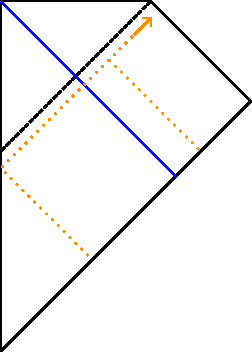
\includegraphics[scale=1]{collapse2}
			\caption{This is the geometry for a black hole made from collapse. Other than in \textbf{Figure \ref{collapse}} the collapsing shell is here shown in blue. The orange dashed line is the late time outgoing wave packet but in backwards evolution. This means, if we would go forwards in time, the arrow would be in the other direction. in seperates because some of it gets reflected off the shell and some goes through the shell.} \label{collapse2}
		\end{center}
	\end{figure}